%!TEX program = xelatex

\documentclass[12pt,a4paper]{article}
\usepackage{xeCJK}
\usepackage{amsmath}
\setmainfont{Times New Roman}
\usepackage{setspace}
\usepackage{caption}
\usepackage{graphicx, subfig}
\usepackage{float}
\usepackage{listings}
\usepackage{booktabs}
\usepackage{setspace}%使用间距宏包
\usepackage{mathtools}
\usepackage{amsfonts}

\begin{document} 
\title{homework4}
	\author{11611118 郭思源}  

\section{Problem 1}
\textbf{Question: State and verify the Lagrange Interpolation Theorem.}

\begin{spacing}{1.5}%%行间距变为double-space
\subsection{What is Lagrange Interpolation Theorem?}
\noindent In numerical analysis, \textbf{Lagrangian interpolation} is a polynomial interpolation method named after French 18th century mathematician Joseph Lagrange. Many practical problems use functions to represent some kind of internal connection or law, and many functions can only be understood through experiments and observations. If you observe a physical quantity in practice and get the corresponding observations in several different places, Lagrangian interpolation can find a polynomial that takes the observed value at each observation point. Such a polynomial is called a \textbf{Lagrangian (interpolation) polynomial}. Mathematically,  Lagrangian interpolation gives a polynomial function that happens to traverse several known points on a two-dimensional plane. The Lagrange interpolation method was first discovered by the British mathematician Edward Waring in 1779, and soon after (1783) was discovered again by Leonhard Euler. In 1795, Lagrange published this interpolation method in his book ``Basic Tutorials for Normal Schools'', and his name has since been associated with this method.\\

\noindent 
For a given ${n+1}$ points ${(x_0,y_0), (x_1,y_1),\ldots,(x_n,y_n)}$, there is only one Lagrangian polynomial L corresponding to their number of times not exceeding n. If a polynomial with a higher number of counts is counted, there is an infinite number because all polynomials that differ from L by 
${\lambda(x_0,y_0)(x_1,y_1)\ldots(x_n,y_n)}$ satisfy the condition.

\newpage
\subsection{Definition}
\noindent For a polynomial function, the given ${n+1}$ value points are known:\\
${(x_0,y_0), (x_1,y_1),\ldots,(x_n,y_n)}$\\
Where ${x_{j}}$ corresponds to the position of the argument, \\
and ${y_{j}}$ corresponds to the value of the function at this position.\\

\noindent Assuming that any two different ${x_{j}}$ are different from each other, the \textbf{Lagrangian interpolation polynomial} obtained by applying the Lagrangian interpolation formula is:

\begin{equation}
	L(x) \coloneqq \sum_{j=0}^n y_j \ell_j(x)
\end{equation}\\

\noindent Each of $\ell _{j}(x)$ is a \textbf{Lagrangian basic polynomial} (or \textbf{interpolation basis function}) whose expression is:

\begin{equation}
\begin{aligned}
	\ell_j(x) \coloneqq &\prod_{i = 0,i \not= j}^n 
	\frac{x-x_i}{x_j-x_i} \\
	= &\frac{x-x_0}{x_j-x_0} \ldots
	\frac{x-x_{j-1}}{x_j-x_{j-1}}
	\frac{x-x_{j+1}}{x_j-x_{j+1}} \ldots
	\frac{x-x_n}{x_j-x_n}
\end{aligned}
\end{equation}\\

\noindent The \textbf{Lagrangian basic polynomial} $\ell _{j}(x)$ is characterized by a value of \textbf{1} on ${x_{j}}$ and a value of 
\textbf{0} on other points ${x_{j}}$, ${i\neq j}$.


\newpage
\subsection{Proof of existence}
For a given $n+1$ point: $(x_{0}, y_{0}), \ldots, (x_{n}, y_{n})$, the idea of ​​Lagrange interpolation is to find one at a point $x_{j}$ takes a value of \textbf{1}, while at other points the polynomial $\ell _{j}(x)$ whose value is \textbf{0}. Thus, the polynomial $y_{j}\ell _{j}(x)$ takes the value $y_{j}$ at point $x_{j}$ and \textbf{0} at other points. \\

\noindent And the polynomial 
\begin{equation*}
	L(x) \coloneqq \sum_{j=0}^n y_j \ell_j(x)
\end{equation*}

\noindent can satisfy :
\begin{equation*}
	L(x_{j})=\sum _{{i=0}}^{{n}}y_{i}\ell _{i}(x_{j})
	=0+0+\cdots +y_{j}+\cdots +0
	=y_{j}
\end{equation*}

\noindent Polynomials with a value of \textbf{0} at other points are easy to find, for example:\\
$(x-x_{0})\cdots (x-x_{{j-1}})(x-x_{{j+1}})\cdots (x-x_{{n}})$\\

\noindent It takes the value $(x_{j}-x_{0})\cdots (x_{j}-x_{{j-1}})(x_{j}-x_{{j+ 1}})\cdots (x_{j}-x_{{n}})$ at point $x_{j}$.\\

\noindent Since $x_{i}$ has been assumed to be different from each other, the above value is not equal to zero. Thus, by dividing the polynomial by this value, you get a polynomial that satisfies "\textbf{1} at $x_{j}$ and \textbf{0} at other points":

\begin{equation*}
\begin{aligned}
	\ell_j(x) \coloneqq &\prod_{i = 0,i \neq j}^k 
	\frac{x-x_i}{x_j-x_i} \\
	= &\frac{x-x_0}{x_j-x_0} \ldots
	\frac{x-x_{j-1}}{x_j-x_{j-1}}
	\frac{x-x_{j+1}}{x_j-x_{j+1}} \ldots
	\frac{x-x_n}{x_j-x_n}
\end{aligned}
\end{equation*}
\newline
\noindent This is the Lagrangian basic polynomial.

\newpage
\subsection{Proof of uniqueness}

There is only one Lagrangian polynomial with a number not exceeding $n$, because the Lagrangian polynomial does not exceed $n$ for any two times: 
$P_{1}$ and $P_{2}$, their difference $P_{1}-P_{ 2}$ is \textbf{0} at all $n+1$ points, so it must be a polynomial $(x-x_{0})(x-x_{{1}})\cdots (x-x_{{n}})$ multiples. \\\\
Therefore, if the difference $P_{1}-P_{2}$ is not equal to \textbf{0}, the number of times must not be less than $n+1$. However, $P_{1}-P_{2}$ is the difference between two polynomials whose number does not exceed $n$, and the number of times does not exceed $n$. So $P_{1}-P_{2}=0$, that is to say $P_{1}=P_{2}$. This proves the uniqueness.

\newpage
\subsection{Geometric property}

Lagrangian basic polynomial $\ell_{0}, \ell_{1}, \cdots, \ell_{n}$ used in Lagrangian interpolation (by a group $x_{0} < x_{1}< \cdots <x_{n}$ determined) can be thought of as a linear space consisting of polynomials of not more than n a set of bases of ${\mathbb {K}}_{n}[X]$.\\

\noindent First, if there is a set of coefficients: $\lambda _{0}, \lambda _{1}, \cdots, \lambda _{n}$\\
let $P=\lambda _{0}\ell _{0}+\lambda _{1}\ell _{1}+\cdots +\lambda _{n}\ell _{n}=\textbf{0}$\\

\noindent Then, on the one hand, the polynomial $P$ is he Lagrangian interpolation polynomial satisfies: \\
$P(x_{0})=\lambda _{0}, P(x_{1})=\lambda _{1}, \cdots, P(x_{n})=\lambda _{n}$ \\

\noindent On the other hand, $P$ is a zero polynomial, so the value is always \textbf{0}. \\
So:\\
$\lambda _{0}=\lambda _{1}=\cdots =\lambda _{n}=\textbf{0}$\\

\noindent This proves that $\ell _{0}, \ell _{1}, \cdots, \ell _{n}$ are linearly independent. At the same time it contains a total of $n+1$ polynomials, which is exactly equal to the dimension of ${\mathbb {K}}_{n}[X]$. So $\ell _{0}, \ell _{1}, \cdots, \ell _{n}$ form a set of bases for ${\mathbb {K}}_{n}[X]$.\\

\noindent The advantage of the Lagrangian basic polynomial as a base is that all polynomials are homogeneous (both nth polynomials).

\newpage
\section{Problem 2}
\textbf{Question: Give some data}
\[
	\begin{array}{r|r}
	t(days) & 7 \quad 14 \quad\ \ 21 \quad\ \ 28 \quad\ \ 35\quad \ \ 42 \\
	\hline
	P(number\;of\;observed\;flies) & 8\quad41\quad133\quad250\quad280\quad297 \\
	\end{array}
\]

\noindent(a) Use the one-term model to fit the data via the least-squares method.\\
(b) Use fifth-order polynomial to interpolate the data.\\
(c) Use low-order polynomial to minimize the $L_1$ norm, $L_2$ norm and $L_\infty$ norm. 

Try second, third order polynomials, respectively.

\subsection{(a)}
\begin{figure}[htbp]
\centering
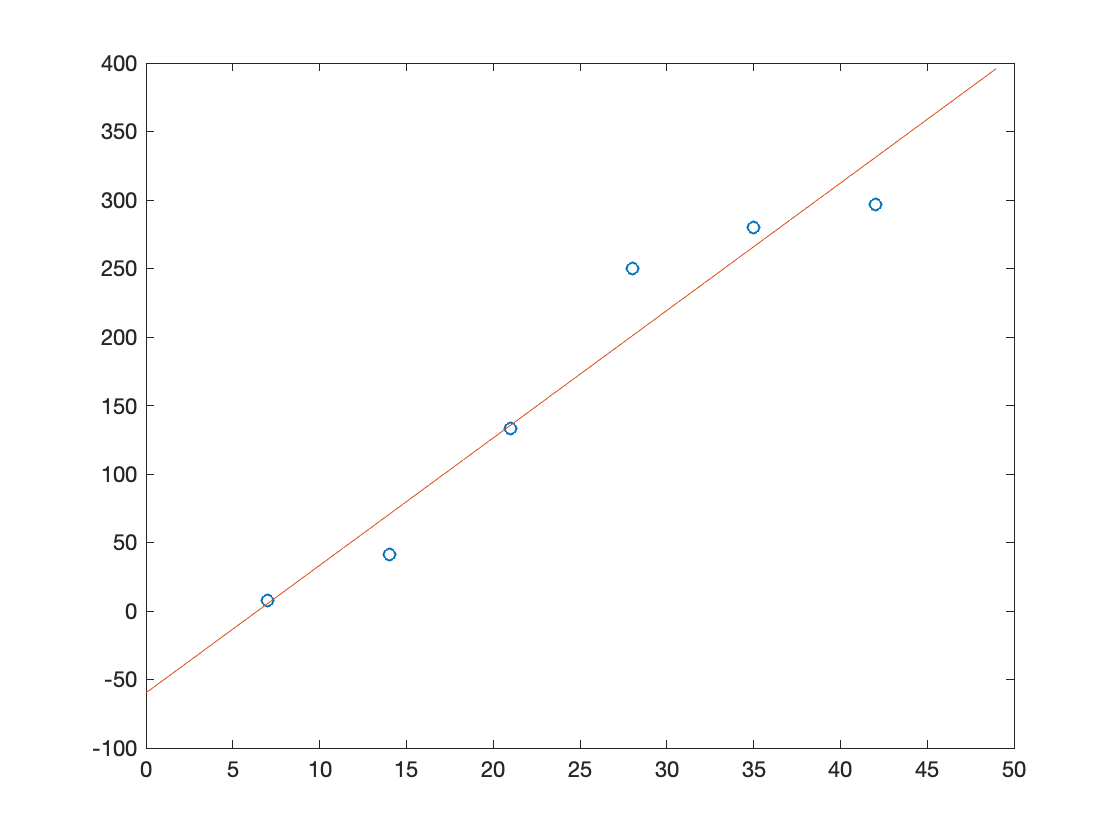
\includegraphics[scale=0.3]{figure/HW4_2_a.png}
\end{figure}

\begin{center}
$y = (2279*x)/245 - 896/15$
\end{center}


\newpage
\subsection{(b)}
\begin{center}
The Lagrangian interpolation is used to interpolate the data:
\end{center}
\begin{figure}[htbp]
\centering
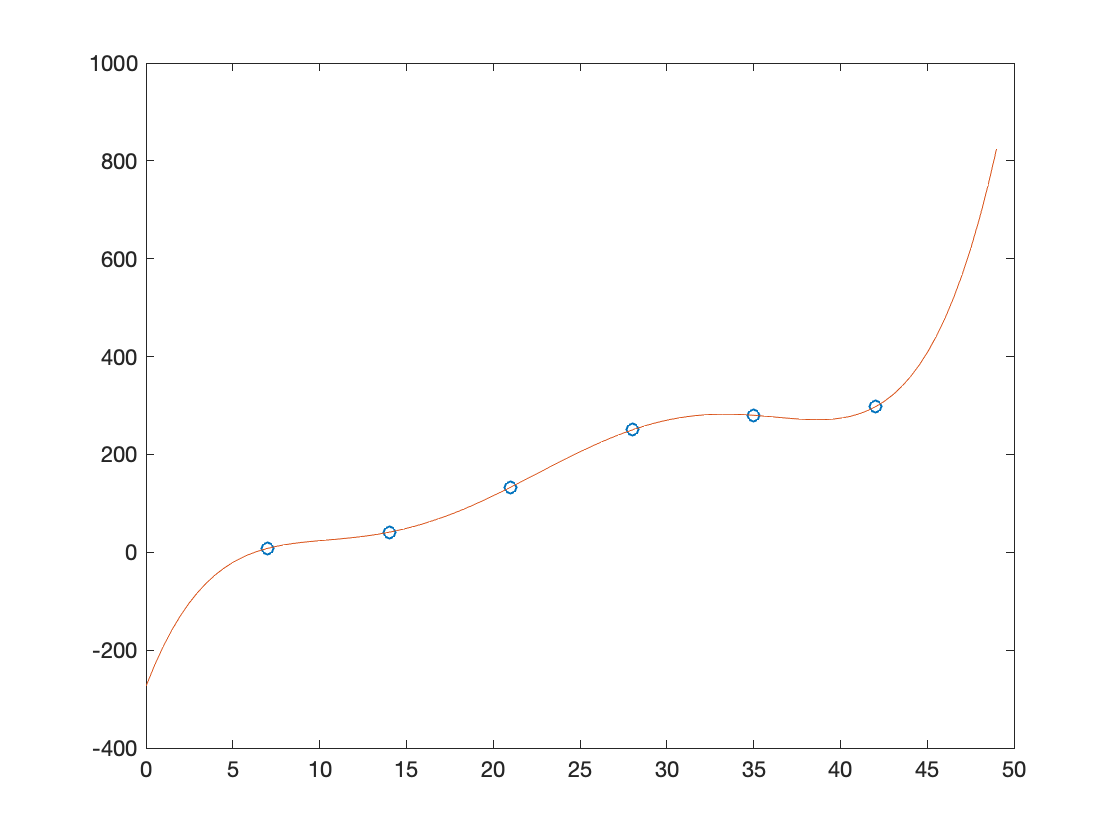
\includegraphics[scale=.3]{figure/HW4_2_b.png}
\end{figure}
\[ \begin{split} 
y = (11*x^5)/84035 &- (145*x^4)/9604 + (1283*x^3)/2058 \\
					&- (2181*x^2)/196 + (9712*x)/105 - 274
\end{split} \]

\newpage
\subsection{(c)}
\begin{figure}[htbp]
\centering
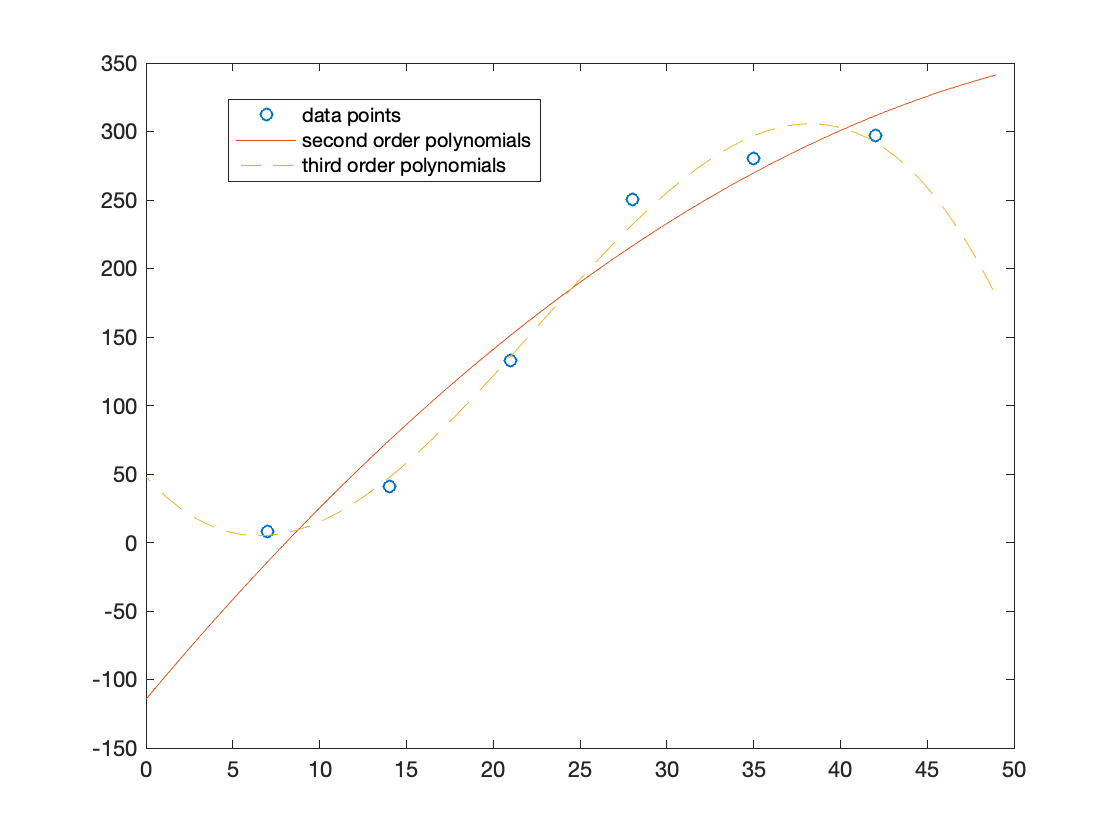
\includegraphics[scale=.3]{figure/HW4_2_c.png}
\end{figure}

Second order polynomials:
\begin{center}
$y = (3714*x)/245 - (41*x^2)/343 - 572/5$
\end{center}

Third order polynomials:
\begin{center}
$y = -(58*x^3)/3087 + (1298*x^2)/1029 - (6185*x)/441 + 48$
\end{center}

\newpage
\subsection{Matlab code}
\begin{lstlisting}[language=matlab]
% HW4_2_a.m
x = [7,14,21,28,35,42];
y = [8,41,133,250,280,297];
p = polyfit(x,y,1);
poly2sym(p)
x1 = linspace(0,49);
y1 = polyval(p,x1);
figure
plot(x,y,'o')
hold on
plot(x1,y1)
hold off

% Hw4_2_b.m
x = [7 14 21 28 35 42];
y = [8 41 133 250 280 297];
x1 = linspace(0,49);
y1 = la(x,y,x1);
plot(x,y,'o')
hold on
plot(x1,y1)
hold off




% la.m
function yy=la(x1,y1,xx)
syms x
n=length(x1);
    for i=1:n
    t=x1;t(i)=[];
    L(i)=prod((x-t)./(x1(i)-t));% L向量用来存放插值基函数
    end
u=sum(L.*y1);
p=simplify(u) % p是简化后的Lagrange插值函数(字符串)
yy=subs(p,x,xx);    % p是以x为自变量的函数,并求xx处的函数值
end

% Hw4_2_c.m
x = [7 14 21 28 35 42];
y = [8 41 133 250 280 297];
p2 = polyfit(x,y,2);
p3 = polyfit(x,y,3);
poly2sym(p2)
poly2sym(p3)
x1 = linspace(0,49);
y2 = polyval(p2,x1);
y3 = polyval(p3,x1);
plot(x,y,'o')
hold on
plot(x1,y2,'-')
plot(x1,y3,'--')
\end{lstlisting}



\end{spacing}


\end{document}